\clearpage
\section{Installation Aktor}\label{sec:Aktor}
Das Aktor-Bord ist die Phisikalische Schnittstellen zu den Elektronischen Verbraucher oder Sensoren. An den Relais K1 bis K4 können ADC 250 Volt und 10 Ampere schalten. An den 0-10 Volt Ausgängen darf einen Maximalen Storm vom 4 mA bezogen werden.
\subsection{Anleitung einrichten}
\begin{figure}[H]
	\centering
	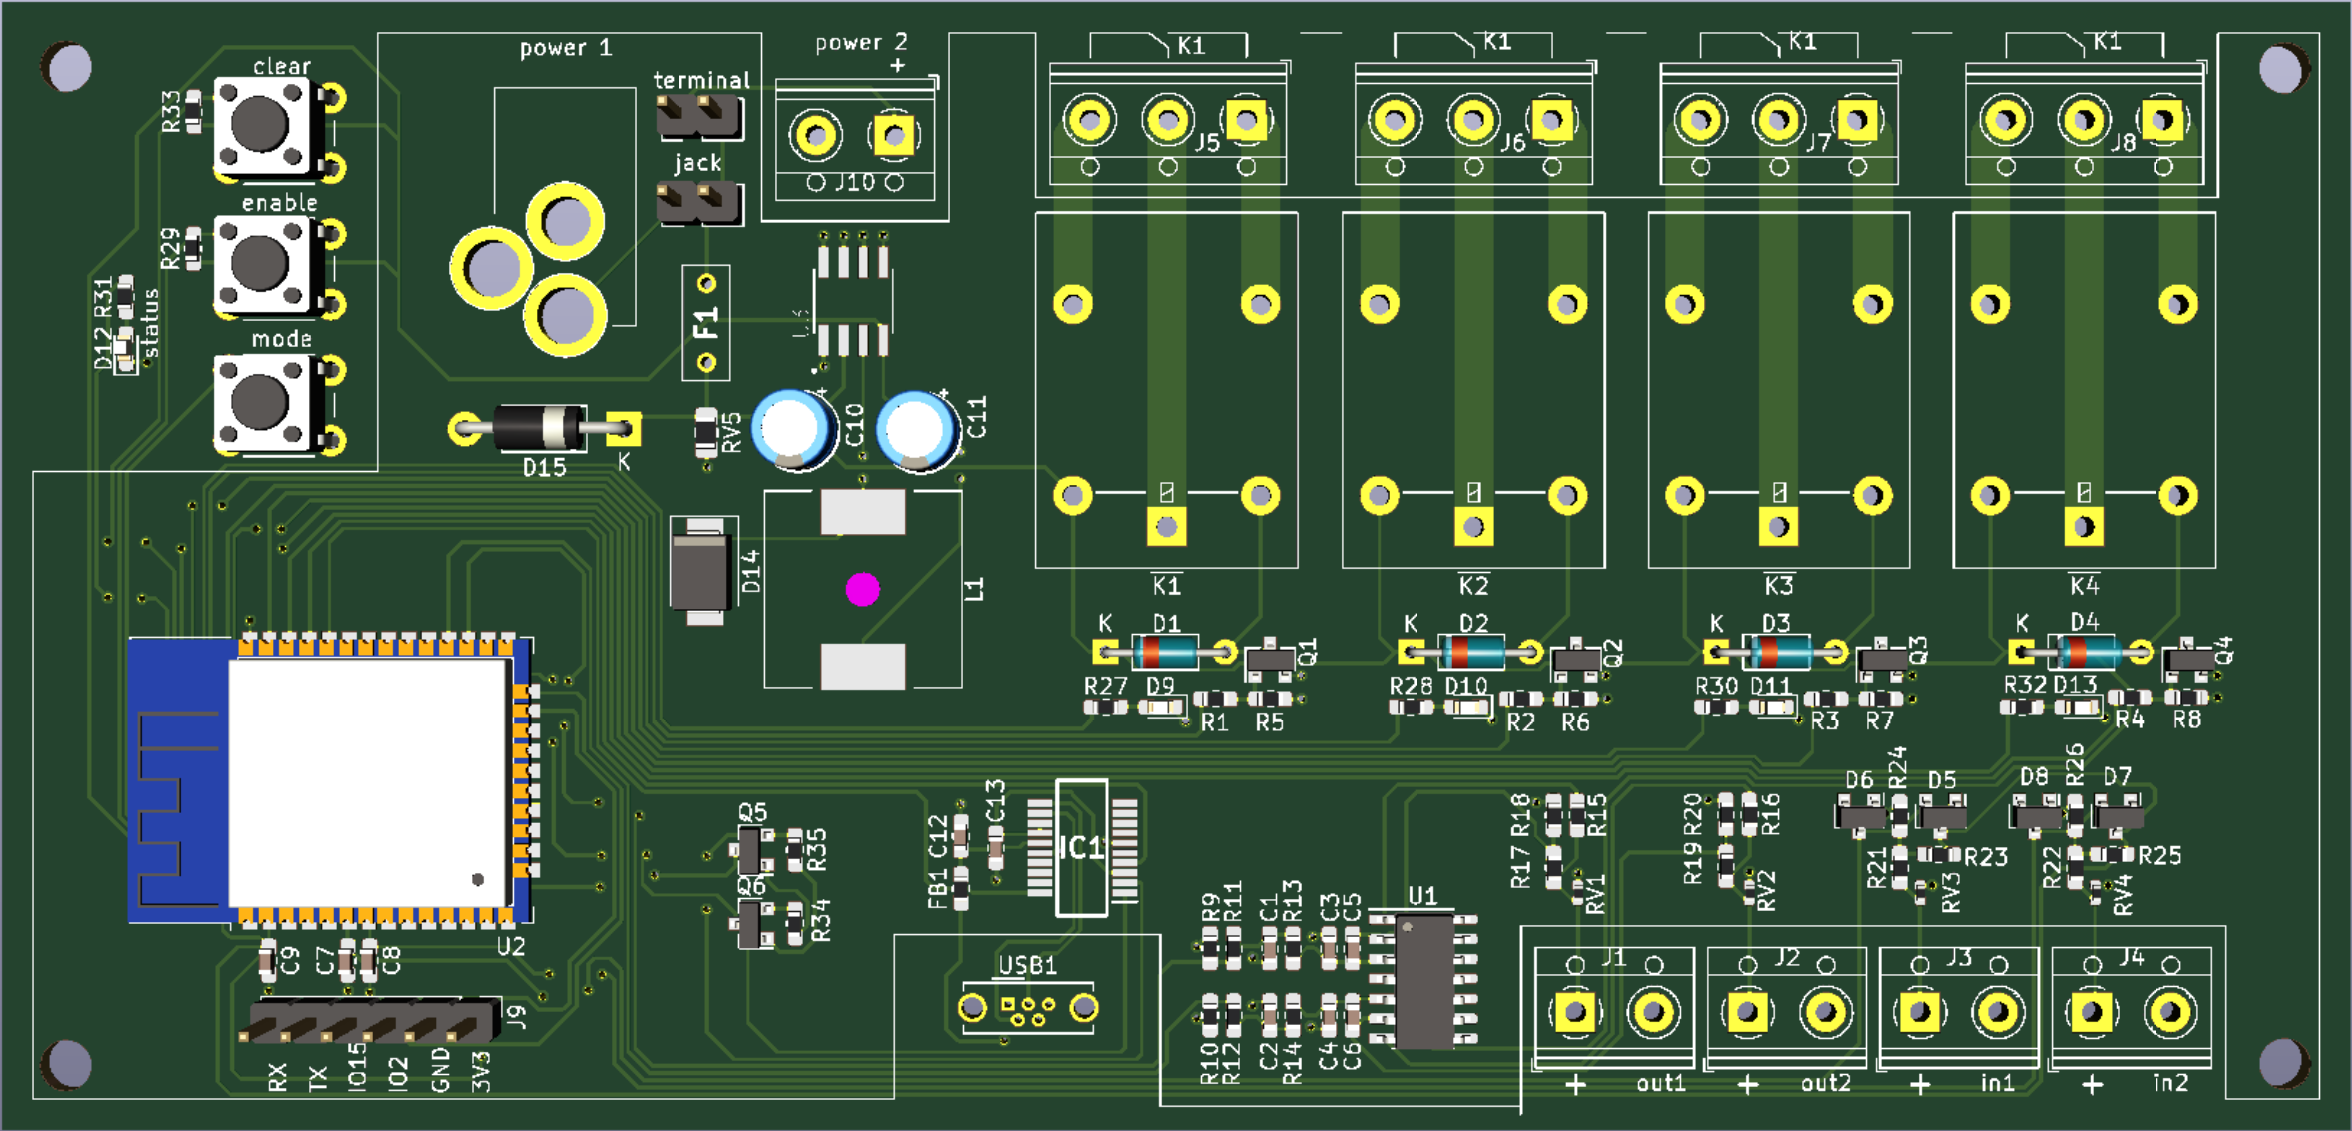
\includegraphics[width=\textwidth]{graphics/Aktorbaustein.png}
	\caption{Aktor Bord} 	
	\label{pic: OSGILayers}
\end{figure} 

\begin{enumerate}
	\item Das Gehäuse des Aktor-Bords soll in eine Haupt- oder Unterverteilung eingebaut werden, wichtig ist zu beachten, dass sich dieser Standort innerhalb der Wlan Reichweite befindet.\\
	\\
	\item Verbraucher wie Leuchten, Storen oder Ventilator können in Schliesser- oder Öffnerbetrieb an den Relais K1 bis K4 angeschlossen werden. Wichtig ist zu beachten dass die Maximale Spannung von 250 Volt ADC und Maximaler Strom von 10 Ampere nicht überschritten wird.\\
		\\
	\item An den out1 und out2 Klemmen können 0-10 Volt Verbraucher angeschlossen werden. Ein Maximaler Strom von 4 mA darf nicht überschritten werden.\\
	\\
	\item An den in1 und in2 Klemmen können 0-10 Volt Sensoren angeschlossen werden.\\
	\\
	\item Als Energieversorgung kann an den Power Klemmen eine 24 V DC Quelle angeschlossen werden. Das Bord kann auch mit einem 24 V DC Hohlstecker verbunden werden.
\end{enumerate}

\subsection{Inbetriebnahme}
Sobald das Aktor-Bord mit Spannung versorgt wird, startet das Configportal des Bords. Mit einem beliebigen Gerät kann im nach einem Wlan Netzwerk gesucht werden. Das Netzwerk hat den Namen "Aktor" gefolgt von der 10 Stelligen Chip-ID des Mikrocontrollers. 
 
\begin{figure}[H]
	\begin{center}
	\begin{minipage}[b]{.3\linewidth} % [b] => Ausrichtung an \caption
		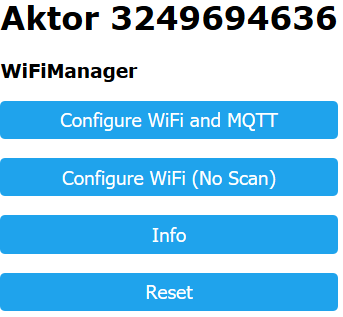
\includegraphics[width=\textwidth]{graphics/Configportal.PNG}
		\caption{Ansicht Configportal Frontseite}
	\end{minipage}
	\hspace{.1\linewidth}% Abstand zwischen Bilder
	\begin{minipage}[b]{.3\linewidth} % [b] => Ausrichtung an \caption
		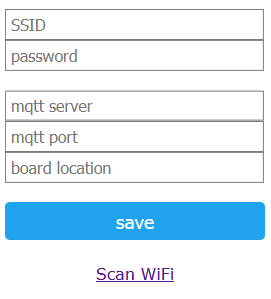
\includegraphics[width=\textwidth]{graphics/Configportal2.PNG}
		\caption{Parameter Config}
	\end{minipage}
\end{center}
\end{figure}
Mit der Funktion Scan WiFi werden vohanden Netzwerke angezeigt. Wird ein eigener MQTT Server installiert kann an dieser Stelle die IP adresse angegeben der Port ist Default "1883". Die Eingabe bei "board location" wird verwendet um MQTT-topics zu generieren, sie muss also eindeutig sein. Werden mehrere Aktor Bords verbaut unterscheiden sie sich an der "bord location". Mit der Taste "save" werden die Eingaben gesichert un müssen bei einem erneuten Start nicht mehr eingegeben werden. Kann sich das Aktor Bord erfolgreich ins Lokale Netztwerk anmelden, blinkt die Status Led in einem regelmässigen Zyklus. Bei jeder Zustandsänderung der Statusleuchte wird eine Messung an den In1 und In2 durchgeführt. 

\subsection{Programmierung}
Verschiedene Eigenschaften können mit dem Entwicklertool zusätzlich verändert werden wenn der Programmcode des Mikrocontrollers bearbeitet wird. In der nachfolgenden Tabelle sind Default-Konfigurationen enthalten.
\begin{table}[H]
\centering
\begin{tabular}{|l|l|l|}
	\hline 
	Bezeichnung & Variable & Wert \\ 
	\hline 
	Zeit Interwall Messungen & NUM\_SEC & 10 \\ 
	\hline 
	Allgemeiner MQTT-Topic  & MQTT\_SERIAL\_PUB & "data/aktorboard/" \\ 
	\hline 
	Messungen für Mean Wert ADC & I & 100 \\ 
	\hline  
\end{tabular} 	
\end{table}
Werden schnelle Reaktionszeiten vom System verlangt können Funktionen direkt im Programmcode Eingebunden werden. So kann eine Reaktionszeit von 300 ms erreicht werden. In diesem Fall wird in der Funktion callback() definiert, wenn topic "data/sensorboard/s1" empfangen wird wird Relais1 geschalten.
\subsection{Netzwerkeinstellungen ändern}
Soll sich das Aktor Bord in ein anderes Netzwerk anmelden gibt es zwei verschiedenen Möglichkeiten. Wenn während des Startvorgangs die Clear taste betätigt wird, eröffnet der Mikrocontroller das Config-Portal. Das Configportal wird ebenfalls geöffnet wenn das einst eingetragene Netzwerk nicht mehr gefunden wird.

\subsection{Topics}
In Nachfolgenden Tabelle die generierten Topics, welche weiter in Openhab verwendet werden. Als location wurde im Configportal "location" eingetragen.
\begin{table}[H]
	\centering
	\begin{tabular}{|l|l|}
		\hline 
		 Topic  & Funktion  \\ 
		\hline 
		data/aktorboard/location/K1 & Schaltet Relais 1  \\ 
		\hline
		data/aktorboard/location/K2 & Schaltet Relais 2  \\ 
		\hline
		data/aktorboard/location/K3 & Schaltet Relais 3  \\ 
		\hline
		data/aktorboard/location/K4 & Schaltet Relais 4  \\ 
		\hline 
		data/aktorboard/location/A1 & Schaltet 0-10V Output 1  \\ 
		\hline
		data/aktorboard/location/A2 & Schaltet 0-10V Output 2  \\ 
		\hline
		data/aktorboard/location/E1 & Publish 0-10V Input 1  \\ 
		\hline
		data/aktorboard/location/E2 & Publish 0-10V Input 2  \\ 
		\hline
	\end{tabular} 	
\label{tab: MQTT-Topics Aktor}
\caption{MQTT-Topics}
\end{table}
 
 Mit den Topics werden die verschiedenen Anwendungen unterschieden, wobei sich der Zustand mit der Payload unterscheidet. Bei den Relais wird zwischen "ON" und "OFF" unterschieden. Bei den 0-10 Volt Inputs so wie Outputs enthält die Payload den entsprechenden Wert. 
